\chapter{Algorithm comparisons for detection of whiteboard}

The issue of contour recognition and segmentation is as of now not completely looked into range of the science. There exists diverse sort of recognition algorithms which are still used. In dissertation will be try to decrease the time spend for processing the image also decrease the memory usage of the algorithms. In paper will be attempting to diminish the time spend for handling the picture additionally processing the memory use of the calculations. To achieve this goal there may be used algorithms like segmentation tree algorithms, depth-first-search, bit mask etc. Early ways to deal with form recognition go for evaluating the nearness of a limit at a given picture area through nearby estimations. The Roberts, Sobel, and Prewitt administrators identify edges by convolving a grayscale picture with local derivative filters.\cite{Argyle} Marr and Hildreth used zero intersections of the Laplacian of Gaussian operator. The Canny indicator likewise models edges as sharp discontinuities in the brightness channel, adding non-maximum suppression and hysteresis thresholding steps.\cite{Pooja} 

We presented a new approach to detect of digital images under the assumption that either the camera that took the image or sufficiently many images taken by that camera are available. Methods automatically determine the required area without assuming any a priori knowledge. 

\section{Different algorithms and techniques}
As it was mentioned by John Canny ``the aim was to discover the optimal edge detection algorithm. In this situation, an "optimal" edge detector means:
\begin{enumerate}
\item Good detection – the algorithm should mark as many real edges in the image as possible.
\item Good localization – edges marked should be as close as possible to the edge in the real image.
\item Minimal response – a given edge in the image should only be marked once, and where possible, image noise should not create false edges.'' \cite{John}
\end{enumerate}

To satisfy these requirements Canny used the calculus of variations – a technique which finds the function which optimizes a given functional. The optimal function in Canny's detector is described by the sum of four exponential terms, but it can be approximated by the first derivative of a Gaussian.

To satisfy all of these requirements Canny used a system which finds the capacity which streamlines a given utilitarian. The ideal capacity in Canny's indicator is portrayed by the entirety of four exponential terms, however it can be approximated by the principal subsidiary of a Gaussian - the calculus of variations.

The algorithm runs in 5 separate steps:
\begin{enumerate}
\item ``Smoothing: Blurring of the image to remove noise.
\item Finding gradients: The edges should be marked where the gradients of the image has large magnitudes.
\item Non-maximum suppression: Only local maxima should be marked as edges.
\item Double thresholding: Potential edges are determined by thresholding.
\item Edge tracking by hysteresis: Final edges are determined by suppressing all edges that are not connected to a very certain (strong) edge'' \cite{John}
\end{enumerate}

The Canny algorithm is easy-usable, powerfull and very adaptable to various environments. \cite{Marr} Its parameters allow it to be used to recognition of edges of different kind of characteristics depending on the particular requirements of a given implementation. \cite{Heath}

In Figure \ref{fig:original_image} is shown original image. In this paper we tried to experiment all described above algorithms for finding edges. According to results was made several analysis why do each of the algorithms fit and not fit in our case.

\begin{figure}[h]
    \centering
    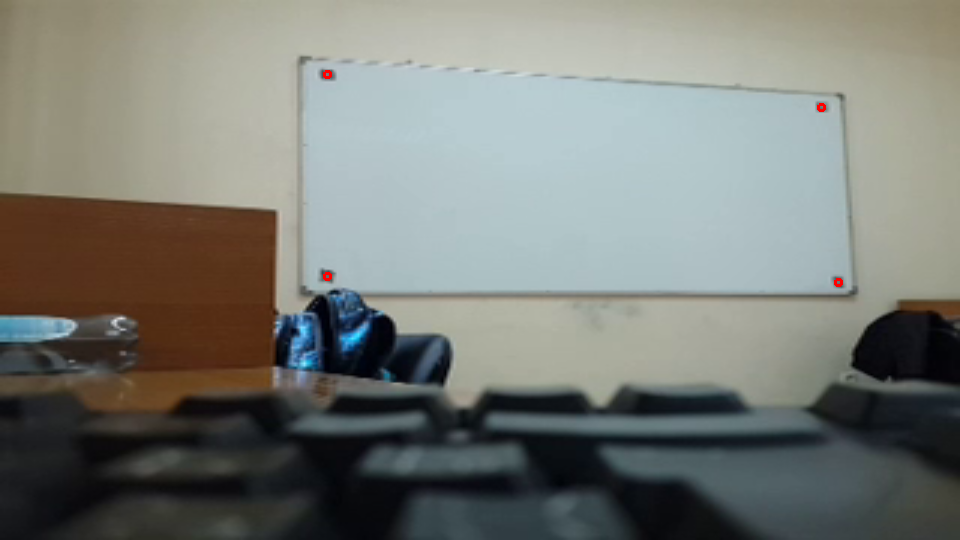
\includegraphics[width=\textwidth]{Figures/original_image}
    \caption{Original Image}
    \label{fig:original_image}
\end{figure}

After trying Canny’s algorithm to find edges of the board we have got the best result among comparing algorithms. In Figure 1.2 is shown the result which was got by running Canny’s algorithms in OpenCV.
The best solution among described algorithms was Canny’s algorithm. Eventhough, this algorithm has disadvantages. The most disadvantage is that in this case we have many candidates. To calculate the corners of the board we will need to perform combination of choosing four patterns from a set of candidates different variants. However preliminary we don’t know the number of candidate it can be very expensive to use this algorithm. One more disadvantage is that there may exists different colors of boards and different brightness of room depending on time when does the video is recording. So, in this case we need to try all the values of lower and upper threshold. It is ineffective because the time we spend for candidate will be multiplied for 255*255(range 0-255) because of need to adjust the threshold each time.

Sobel operator is quite similar to the Prewitt operator, and the modification is to use a weighting factor for the two middle elements:

\begin{equation}
    G_x = (z_7 + 2z_8 + z_9) - (z_1 + 2z_2 + z_3)
\end{equation}
\begin{equation}
    G_y = (z_3 + 2z_6 + z_9) - (z_1 + 2z_4 + z_7)
\end{equation}

This increased value is used to reduce the effect of smoothing by giving more weight to the middle points. Masks used Sobel operator are displayed in the Figure \ref{fig:masks_sobel_operator}.

\begin{figure}[h!]
    \centering
    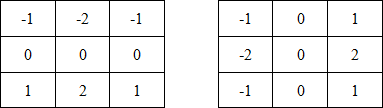
\includegraphics{Figures/masks_sobel_operator}
    \caption{Masks Sobel operator}
    \label{fig:masks_sobel_operator}
\end{figure}

The above masks are used for the components of the gradient. To calculate the gradient of these components must be combined \cite{Vincent}: 
\begin{equation}
    \triangledown f \approx  |G_x| + |G_y|
\end{equation}
\begin{equation}
    f = \sqrt{G_x^2 + G_y^2}
\end{equation}

In Figure \ref{fig:sobel_result} is shown the result which was taken by running Sobel algorithm of find the edges of the baord. Moreover, in Figure \ref{fig:laplasian_result} and Figure \ref{fig:masks_sobel_operator} you can see the corresponding results after applying edge detecting algorithms.

The poorest results were got in Sobel’s algorithm. The main reason for that is that the algorithm works only with horizontal and vertical lines. In our case it is not guaranteed that the camera will be exactly in front of the board and the borders of the board will lay exactly over the x and y axis. In our case the camera can be located in any place of the room not far from the board. To sum up this algorithm is not the best one to use in our application.

\begin{figure}[h]
    \centering
    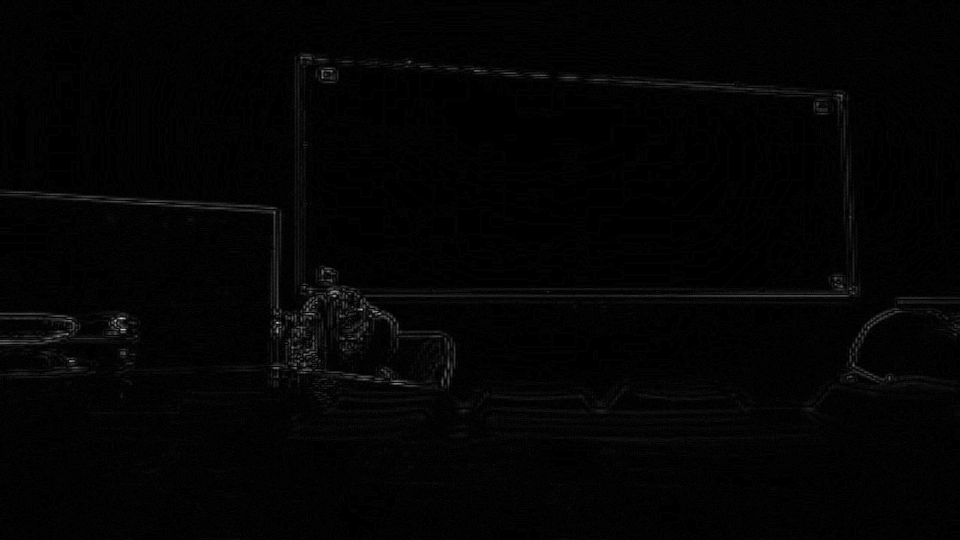
\includegraphics[width=0.7\textwidth]{Figures/laplasian_result}
    \caption{Laplasian algorithm result}
    \label{fig:laplasian_result}
\end{figure}
\begin{figure}[h]
    \centering
    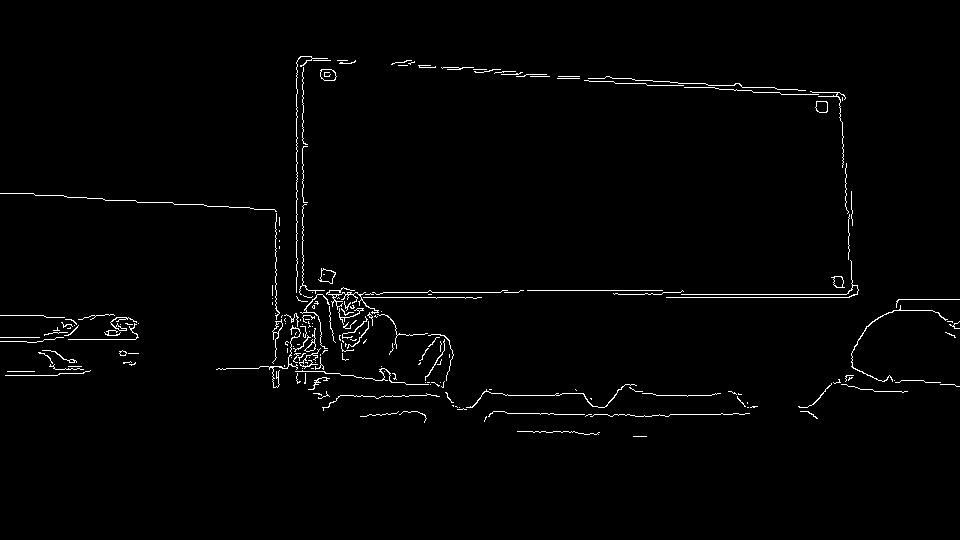
\includegraphics[width=0.7\textwidth]{Figures/canny_result}
    \caption{Canny's algorithm result}
    \label{fig:masks_sobel_operator}
\end{figure}
\begin{figure}
    \centering
    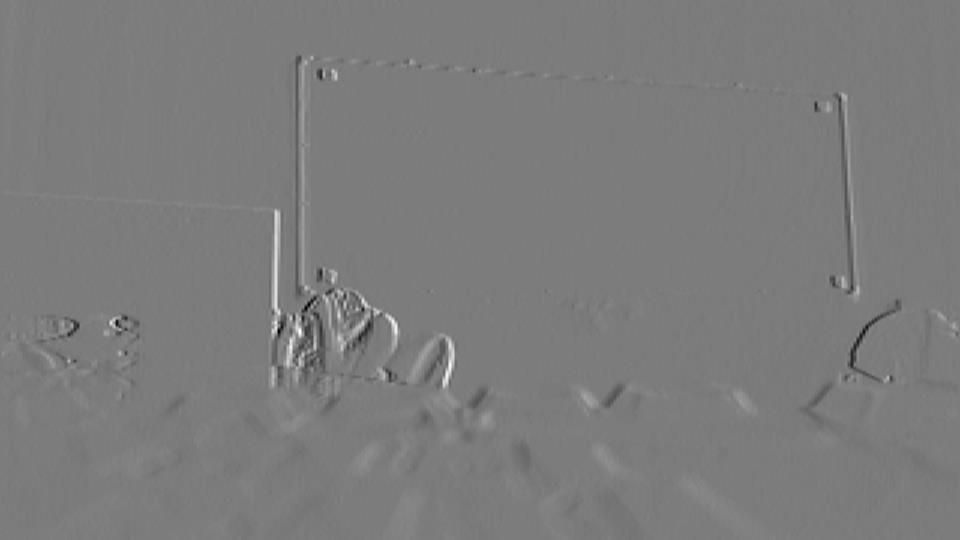
\includegraphics[width=0.7\textwidth]{Figures/sobel_result}
    \caption{Sobel algorithm result}
    \label{fig:masks_sobel_operator}
\end{figure}

Another derivative operator is Laplacian Operator which is used widely to discover and recognize edges in a picture outlines. In this cover we have two further portrayals one is Positive Laplacian Operator and other is Negative Laplacian Operator. The major and the normal distinction amongst Laplacian and different operators like Prewitt, Sobel, Robinson and Kirsch is that these all are first request subsidiary covers, all things considered Laplacian is a second request subordinate. 

Another difference amongst Laplacian and different operators are that not all different operators Laplacian didn't take out edges in a specific heading yet it take out edges in taking after classification.

In Positive Laplacian we have standard mask in which center element of the mask should be negative and corner elements of mask should be zero. \cite{Huertas}
 
Disadvantage of these algorithms is that the boards of the board and lines in the final image are very week and it contains many noises which is really obstacle in our image processing process. This algorithm works weaker than Canny’s algorithms.

Robert’s algorithm takes the domain 3x3, shown in the figure below (see Fig. \ref{fig:neighborhood_within_image}), represents the brightness values in the neighborhood of a pixel.

\begin{figure}[h]
    \centering
    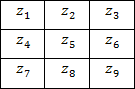
\includegraphics{Figures/neighborhood_within_image}
    \caption{3x3 neighborhood within the image}
    \label{fig:neighborhood_within_image}
\end{figure}

One of the easiest ways to find the first partial derivatives at the point image is to apply the following cross-gradient operator Roberts \cite{Seif}: 

\begin{equation}
    G_x = (z_9 - z_5)
\end{equation}
\begin{equation}
    G_y = (z_8 - z_6)
\end{equation}

These derivatives can be realized by processing the entire image using the operator masks described in Figure \ref{fig:masks_operator_roberts}, using the procedure of filtering, as previously described.

\begin{figure}[h]
    \centering
    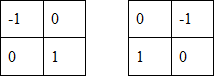
\includegraphics{Figures/masks_operator_roberts}
    \caption{Masks operator Roberts}
    \label{fig:masks_operator_roberts}
\end{figure}

Implementation masks 2x2 is not very convenient, since they have no explicit central element that significantly affects the result of the filtering. But this "minus" generates a very useful feature of this algorithm - high speed image processing. Convert each pixel Roberts cross operator may show a non-zero derivative of the image along the diagonal, and a combination of the transformed images may be regarded as the gradient of the two upper pixels in the bottom two. Roberts operator is still used for computing speed, but it pales by comparison with the alternatives with its significant problem of sensitivity to noise. He gives a finer line than other methods of isolation boundaries. Sometimes it is called "filter Roberts."\cite{Seif}

Prewitt operator, as well as the operator Roberts operates 3x3 image area shown in figure, only the use of such a mask is given other expressions: 

\begin{equation}
    G_x = (z_7 + z_8 + z_9) - (z_1 + z_2 + z_3)
\end{equation}
\begin{equation}
    G_y = (z_3 + z_6 + z_9) - (z_1 + z_4 + z_7)
\end{equation}

In these formulas, the difference between the amounts on the top and bottom rows of 3x3 neighborhood is an approximate value of the derivative along the axis x, and the difference between the sums of the first and last columns of this neighborhood - the derivative along the axis y. 

In simple terms, the operator calculates the gradient of the image intensity at each point. It gives the direction of the biggest possible increase from light to dark and the rate of change in that direction. The result therefore shows how "abruptly" or "smoothly" the image changes at that point. Therefore how likely it is that part of the image represents an edge, as well as how that edge is likely to be oriented. In practice, the magnitude calculation is more reliable and easier to interpret than the direction calculation as it is likelihood of an edge. \cite{Roberts}

In basic terms, the operator computes the inclination of the picture at every point. It gives the bearing of the greatest conceivable increment from bright to dark and the rate of alter in that course. The outcome accordingly demonstrates how "abruptly" or "smoothly" as it was discussed in \cite{Roberts} the picture changes by then. Hence how likely it is that part of the image represents an edge, and additionally how that edge is likely to be oriented. In practice, the magnitude calculation is more solid and less demanding to translate than the bearing estimation as it is probability of an edge.

As it is mentioned in \cite{Raman} ``Mathematically, the gradient of a two-variable function (here the image intensity function) is at each image point a 2D vector with the components given by the derivatives in the horizontal and vertical directions. At each image point, the gradient vector points in the direction of largest possible intensity increase, and the length of the gradient vector corresponds to the rate of change in that direction. This implies that the result of the Prewitt operator at an image point which is in a region of constant image intensity is a zero vector and at a point on an edge is a vector which points across the edge, from darker to brighter values.''

\section{Detection using consecutive frames}

Finally we came to decision to use four figures as a rectangle at the four corners of the board. First the image takes from the normal state where the rectangles are not signed at the board. After the taking the static image of the board the person who is testing need to close the camera with his/her hand informing that the camera need to work with the new frames where will be the four rectangles at four corners of the board. After the rectangles will be drawn to the board the camera takes the final image and makes the subtraction with the first original static image. After, the difference between images will be obvious so there will appear only four rectangles which will make much easier to work with image. This image of difference is considered as an image which need to be scanned. 

More detailed description of rectangle finding algorithm. There are several stages:
\begin{enumerate}
\item Take difference before and after hand cover
\item Divide into components
\item Bound by box
\item Recognize boxes as rectangle
\item Comparing of the area of rectangles
\end{enumerate}

First, to take difference before and after the hand cover the application collects last 5 motionless static frames and also collects 5 motionless static frames after the hand cover. Then if there exists such frames their differences uses as a further image for determining the rectangles. 

Second, we need to divide all this points into components to determine that they lay in different places. To decrease the number of components we used morphological operations. In short: A set of operations that process images based on shapes. Morphological operations apply a structuring element to an input image and generate an output image.

The most basic morphological operations are two: Erosion and Dilation. They have a wide array of uses, i.e.:
\begin{itemize}
    \item Removing noise
    \item Isolation of individual elements and joining disparate elements in an image
    \item Finding of intensity bumps or holes in an image
\end{itemize}

Both of morphological operations can be used to decrease the number of components. Using dilation or erosion we can connect into one component the components which are located very close to each other.

After the morphological operations it is more comfortable to divide it into different component. To divide it is possible to use algorithms like depth first search algorithm or breadth first search algorithm. In fact, we will be producing a series of detours, first run in the first round the top, and all the vertices, while he walked - form the first connected component. Then we find the first of the remaining vertices that have not yet been visited, and run circumvention of it, thus finding a second connected component. And so on, until all the vertices become marked.

The total amount to the asymptotic behavior of O (n + m): in fact, this algorithm will not run on the same vertex twice, which means that each edge will be seen exactly twice (at one end and the other end).\cite{Thomas}

To find components it is more convenient to use DFS algorithm. However we work with large images and it is important to spend less memory and time for handling the images. In case of DFS algorithm the required memory will be the length of the deepest component of the graph. In BFS algorithm the size of memory is fixed. The memory size will be (n*m) the number of pixels. However in our case the size of rectangle is not going to be very large we used DFS algorithm.

After the running DFS algorithm we will got n(close to number 4) components. Then, after dividing all points into different component we need to draw bounding box to determine is it rectangle or not. Because we are interested only on rectangles we need to check each component for rectangle. For determining the rectangle there exists several solutions. One of the best solution is to draw a bounding box over the each component and then to work with ideal candidate for a rectangle. In our case the bounding box of each component will be the most left, right, top bottom lines of the component. It is obvious that one component is a collection of pixels. To determine the most left and most right coordinates on x axis and the most top and most bottom y axis coordinates of the pixel we just run through all the points of the component and for each pixel we will try to find the minimum and maximum x and y values. This four values (minimum x, y and maximum x, y) will be borders of the bounding box. 

We will run this bounding box algorithm for each component. After the getting all bounding boxes we will check each of them for rectangle. After, only the best candidates will left. There are several ways to check the candidates whether they are the four corners of the board: the areas of the rectangles must be close to each other, the length of diagonals must be close to each other.

To calculate the areas of rectangles it is enough to multiply the absolute differences between maximum and minimum x and y values. The formula of calculation is shown as follows:

\begin{equation}
    Sarea = (Xmax - Xmin) \cdot (Ymax - Ymin)
\end{equation}

To calculate the diagonals length’s we need to put all the candidates for four corners of the board. To perform it we can just sort all components by its coordinates and just begin to locate component which is located at the top left then top right then bottom left then bottom right.

After we will compare all diagonals between each other and get the best four rectangles which will be the four corners of the board.

The number of combinations to compare the diagonals can be calculated by the following formula: 
\begin{equation}
    T = C_n^4
\end{equation}
Where $T$ is the number of combinations and n is the number of candidates (components). 

How mentioned above we need to come up with three stages to get the actual board image which will be sent to the server. After the first step we get the image like in Figure \ref{fig:captured_image}

\begin{figure}[h]
    \centering
    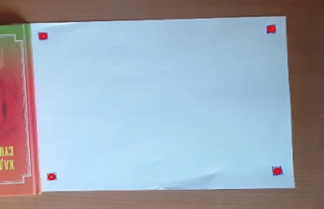
\includegraphics{Figures/captured_image}
    \caption{Captured image in testing}
    \label{fig:captured_image}
\end{figure}

\begin{figure}[h]
    \centering
    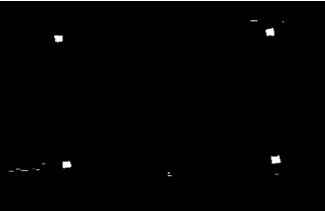
\includegraphics{Figures/after_taking_difference}
    \caption{The image after taking difference}
    \label{fig:after_taking_difference}
\end{figure}


In this image we can see that algorithm has detected four corners of the paper and its ready to perform next step in the way of getting the final image. But to get this image first we took difference between last and previous images and further make search for rectangle polygons from the image. The difference image looks like in Figure \ref{fig:after_taking_difference}

We have a binary image that contains from black and white pixels. We are interested only in white pixels. So in our case we can have a lot of candidates for being the corners of rectangle, however we can easily eliminate all the unnecessary white points. Algorithm is as follows. First, we make an erosion on the image, because of this the points that are close to each other joins and there would be any gap. \cite{Ruchika} Then, we can run the depth-first-search algorithm to find the connected components. Then we identify for each connected component its bounding box, top-left, top-right, bottom-left, bottom-right corners for each component. So then we calculate the proportion of the area with this rectangle that is created by bounding box. We can make some thresholding for that. So if there is a lot of candidates we will take first four with a maximal area. In figure 6.3 is shown another results of applying the above algorithm

\begin{figure}[h]
    \centering
    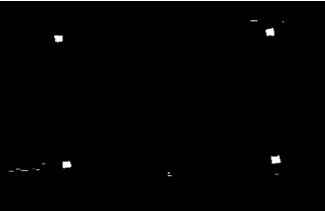
\includegraphics{Figures/after_taking_difference}
    \caption{Result of described algorithm on Figure \ref{fig:original_image}}
    \label{fig:after_taking_difference}
\end{figure}


In this case we got the minimal number of candidates. The number of candidates and not need to adjust threshold was the main advantage over the Canny’s algorithm. Like in any algorithm it has disadvantages too. They are: the camera need to be fixed in one place; Person needs to close with his hand the camera. However we considered that the camera will be static we can accept that in our case the best algorithm is our algorithm. In a Table \ref{tab:comparison_table} we can see the comparison between Canny’s algorithm and our algorithm. The number of candidates with average quality of threshold is calculated using the results of image in Figure \ref{fig:original_image}. Our algorithm is beating well-known Canny’s algorithm with many parameters. However the main drawbacks of our algorithm is the number of frames that needed to act properly.

\begin{longtable}[t]{|p{0.35\textwidth}|p{0.30\textwidth}|p{0.25\textwidth}|}
\caption{Comparison Table}\label{tab:comparison_table} \\
	\hline
	\textbf{Methods} & \textbf{Canny's algorithm} & \textbf{Our algorithm} \\
	\hline
	\endhead
	Thresholding 
	& Required
	& Not required\\
	\hline
	Number of candidates with avarage quality of threshold 
	& 14
	& 5 \\
	\hline
	Exactly identified with a set of candidates 
	& NO
	& YES\\
	\hline
	Number of 4 candidate set 
	& $C(_{14}^4) = 1001$
	& $C(_5^4) = 5$\\
	\hline
	Required frame number 
	& 1
	& 2\\
	\hline
	Candidate finding time complexity 
	& O(N*M)
	& O(N*M)\\
	\hline
\end{longtable}

After the getting the four candidates as a rectangle we can perform the matrix transformation algorithm. This algorithm is fully implemented in openCV. From this final image we can make further image transmission operations. The image is ready to be transmitted. 
